\documentclass[letterpaper, 12pt]{article}

\usepackage[top=2.5cm, bottom=2.5cm, left=2cm, right=2cm]{geometry}
\usepackage{amsmath, amsfonts, amssymb, amsthm}
\usepackage{graphicx}

\def\e{\text{e}}
\def\L{\mathcal{L}}
\def\i{\text{i}}
\def\d{\text{d}}
\def\R{{\mathbb{R}}}
\def\C{{\mathbb{C}}}

\title{Solving parabolic PDEs in parallel via time discretization using Laplace transforms}
\author{Kyle Geyser and Dylan Denning}
\date{\today}

\begin{document}
	\begin{titlepage}
		\maketitle
		
		\vspace{3cm}
 
		\begin{abstract}
			For this project, we will outline a method to solve inhomogeneous parabolic partial differential equations in parallel. This will be accomplished by removing the time dependence of the equations by transforming the problem into a differential equation in the space-frequency setting through a Laplace transformation. For each discrete frequency, an independent spatial problem exists which can be solved with a finite difference method for numerically approximating solutions to differential equations. Due to the independence of the spatial problems, many problems can be solved at the same time in a parallel environment. This paper will further explain the details required to produce accurate results for such problems.
		\end{abstract}
	\end{titlepage}
	
	\section*{Problem Description}
		The problems we will consider are of the form
		$$u_t+Au=f(t),\hspace{4mm}\text{for }t>0,\hspace{4mm}\text{with }u(0)=u_0$$ \\
		where $A$ is the second-order differential operator ($\nabla^2$) with Dirichlet boundary conditions and $u_0$ and $f(t)$ are given.
		Note: all functions above have implied spatial terms based on the dimensionality of the problem

	\section*{Approach}
		To remove the time dependece of the problem, we transform the equation with a Laplace transform defined by
		$$w(z):=\L\{u\}=\hat{u}(z)=\int_0^\infty\e^{-zt}u(t)\d t$$
		To get a solution for $u$, we must take an inverse Laplace transform of $w$ defined by
		$$u(t)=\frac{1}{2\pi\i}\int_\Gamma\e^{zt}w(z)\d z$$	
		where $\Gamma$ is a deformed contour in the complex plane, assuming $w(z)$ can be continued analytically. 
		$$\Gamma=\{z:z=\varphi(y)+\i\sigma y, y\in\R, y\text{ increasing}\}\subset S, S=\{z\in\C:|\arg z|<\delta, z\neq 0\}, \delta\in(\pi/2,\pi)$$
		
	\section*{Approach and Methodology}
	\hspace{5mm} We will begin our studies with producing a working serial version of the algorithm for ordinary differential equations with known solutions, with which we can then compare computed results. Following successful completion of said serial algorithm, we will make the necessary adjustments as to allow for partial differential equation computations, still performing all computations in serial. Once a fully working serial version of the code is completed, we will proceed to parallelize the algorithm to produce our intended final result. By approaching the problem with this methodology, we can work in steps in which we feel comfortable. Between each step, should we need outside guidance, we can approach Dr. Ganesh with any problems we are having, while still showing that we are making progress toward a final production. Throughout the time spent working through these milestones, we can further our knowledge on the subject matter by continuing to digest more of the material in the provided article\cite{sheen03} as well as learn new material in the field of numerical solutions to PDEs through Dr. Ganesh's private lectures.
	
	\subsection*{Expected Outcome}
	\hspace{5mm} Since we are replicating the process in the article by Sheen, Sloan, and Thom\'{e}e, we expect to get the same results the authors show in section 6 (Numerical examples) in their paper.\cite{sheen03}
	
	\subsection*{Tables and Plots}
	
	\subsubsection*{Table 1} \small\textit{Error and apparent order of convergence for Example 1 with $N=10,20,40$,\\ and $80$ for $\tau=0.5$} \\\\
	\normalsize
	\begin{tabular}{r||rrrrrrr}
		\hline
		$t$  &$\epsilon_{10}$  &$\epsilon_{20}$  &$\rho_{20}$  &$\epsilon_{40}$  &$\rho_{40}$  &$\epsilon_{80}$  &$\rho_{80}$ \\ 
		\hline
		0.2    &3.715E-04    &2.018E-04         &0.88    &3.574E-04        &-0.82    &3.451E-04         &0.05 \\ 
		0.4    &4.808E-04    &1.654E-04         &1.54    &3.972E-05         &2.06    &1.710E-06         &4.54 \\ 
		0.6    &1.704E-05    &2.586E-05        &-0.60    &9.553E-06         &1.44    &1.705E-06         &2.49 \\ 
		0.8    &1.441E-05    &1.837E-07         &6.29    &1.175E-06        &-2.68    &3.131E-07         &1.91 \\ 
		1.0    &9.086E-06    &1.158E-06         &2.97    &4.299E-08         &4.75    &4.452E-08        &-0.05 \\ 
		1.2    &1.480E-06    &2.628E-07         &2.49    &2.781E-08         &3.24    &5.071E-09         &2.46 \\ 
		1.4    &5.214E-06    &2.419E-08         &7.75    &9.365E-09         &1.37    &2.872E-10         &5.03 \\ 
		1.6    &9.582E-06    &2.534E-08         &8.56    &1.248E-09         &4.34    &6.188E-11         &4.33 \\ 
		1.8    &1.545E-05    &7.777E-09        &10.96    &1.674E-10         &5.54    &2.650E-11         &2.66 \\ 
		2.0    &2.305E-05    &7.890E-09        &11.51    &1.221E-10         &6.01    &5.444E-12         &4.49 \\ 
		3.0    &9.117E-05    &2.193E-08        &12.02    &1.247E-13        &17.42    &6.523E-16         &7.58 \\ 
		4.0    &2.640E-04    &6.540E-08        &11.98    &5.787E-15        &23.43    &6.939E-18         &9.70 \\ 
		\hline
	\end{tabular}
	
	\subsubsection*{Table 2} \small\textit{Errors and apparent orders of convergence for Example 1 with $N=40$\\ and $80$ for $\tau=0.25$ and $1.0$} \\\\
	\normalsize
	\begin{tabular}{r||rrr|rrr}
			     &             &$\tau = 0.25$		  &	 	  	 &             &$\tau = 1.0$    	&		  \\
		\hline
		$t$  &$\epsilon_{40}$  &$\epsilon_{80}$  &$\rho_{80}$  &$\epsilon_{40}$  &$\epsilon_{80}$  &$\rho_{80}$ \\ 
		\hline
		0.2    &1.954E-05    &6.513E-07         &4.91    &4.940E-03    &2.792E-03         &0.82 \\ 
		0.4    &4.151E-07    &1.258E-07         &1.72    &1.344E-03    &1.060E-03         &0.34 \\ 
		0.6    &9.456E-09    &1.612E-09         &2.55    &7.211E-04    &3.211E-04         &1.17 \\ 
		0.8    &7.712E-10    &2.510E-11         &4.94    &6.373E-05    &2.477E-05         &1.36 \\ 
		1.0    &4.394E-10    &1.504E-12         &8.19    &6.359E-05    &3.183E-05         &1.00 \\ 
		1.2    &4.342E-10    &2.195E-14        &14.27    &2.678E-05    &3.323E-06         &3.01 \\ 
		1.4    &1.454E-09    &1.832E-15        &19.60    &8.530E-07    &2.766E-06        &-1.70 \\ 
		1.6    &2.700E-09    &4.163E-16        &22.63    &4.399E-06    &8.962E-07         &2.30 \\ 
		1.8    &4.220E-09    &4.441E-16        &23.18    &1.281E-06    &1.798E-07         &2.83 \\ 
		2.0    &6.075E-09    &5.829E-16        &23.31    &3.676E-07    &1.596E-07         &1.20 \\ 
		3.0    &2.355E-08    &2.318E-15        &23.28    &3.466E-09    &1.814E-09         &0.93 \\ 
		4.0    &7.010E-08    &6.994E-15        &23.26    &6.142E-10    &3.219E-11         &4.25 \\ 
		\hline
	\end{tabular}
	
	\subsubsection*{Table 3} \small\textit{Error and apparent order of convergence for Example 2 with $N=20$ and\\$m=10,20,40$, and $80$ for $\tau=0.5$} \\\\
	\normalsize
	\begin{tabular}{r||rrrrrrr}
		\hline
		$t$  &$\epsilon_{10}$  &$\epsilon_{20}$  &$\rho_{20}$  &$\epsilon_{40}$  &$\rho_{40}$  &$\epsilon_{80}$  &$\rho_{80}$ \\ 
		\hline
		0.2    &1.269E-02    &2.102E-02        &-0.73    &2.381E-02        &-0.18    &2.450E-02        &-0.04 \\ 
		0.4    &2.140E-02    &8.455E-03         &1.34    &5.226E-03         &0.69    &4.416E-03         &0.24 \\ 
		0.6    &1.522E-02    &3.802E-03         &2.00    &9.256E-04         &2.04    &2.070E-04         &2.16 \\ 
		0.8    &1.212E-02    &2.912E-03         &2.06    &6.515E-04         &2.16    &8.384E-05         &2.96 \\ 
		1.0    &9.506E-03    &2.351E-03         &2.02    &6.009E-04         &1.97    &1.661E-04         &1.86 \\ 
		1.2    &7.370E-03    &1.811E-03         &2.02    &4.520E-04         &2.00    &1.141E-04         &1.99 \\ 
		1.4    &5.859E-03    &1.470E-03         &2.00    &3.650E-04         &2.01    &8.993E-05         &2.02 \\ 
		1.6    &5.148E-03    &1.276E-03         &2.01    &3.186E-04         &2.00    &7.977E-05         &2.00 \\ 
		1.8    &4.663E-03    &1.176E-03         &1.99    &2.937E-04         &2.00    &7.348E-05         &2.00 \\ 
		2.0    &4.468E-03    &1.114E-03         &2.00    &2.783E-04         &2.00    &6.958E-05         &2.00 \\ 
		3.0    &3.091E-03    &7.691E-04         &2.01    &1.927E-04         &2.00    &4.823E-05         &2.00 \\ 
		4.0    &1.825E-03    &4.533E-04         &2.01    &1.133E-04         &2.00    &2.854E-05         &1.99 \\ 
		\hline
	\end{tabular}
	
	\subsubsection*{Table 4} \small\textit{Number of cores vs. runtime(in seconds) for $N=50,000$\\ and $m=250,000$} \\\\
	\normalsize
	\begin{tabular}{r||r|r}
	\hline
		Cores              &Sayers Lab                     &Mio \\ 
	\hline
		  1.0      &3661.0877999999998      &2245.8103000000001 \\ 
		  2.0      &1918.2696000000001      &1182.6335999999999 \\ 
		  4.0               &1021.9571      &636.83158000000003 \\ 
		  8.0      &474.32260000000002               &348.26038 \\ 
		 16.0      &264.32758000000001      &164.24718999999999 \\ 
		 32.0               &153.50402      &80.234003999999999 \\ 
		 64.0      &84.893333999999996      &43.834428000000003 \\ 
		128.0                     &N/A      &21.293009999999999 \\ 
		256.0                     &N/A      &16.503080000000001 \\ 
		512.0                     &N/A      &23.166782000000001 \\ 
		\hline
	\end{tabular}
	
	\subsubsection*{Plot 1} \small\textit{Plot of Table $4$ data $(lg(cores)$ vs. $lg(runtime))$} \\
	\normalsize
	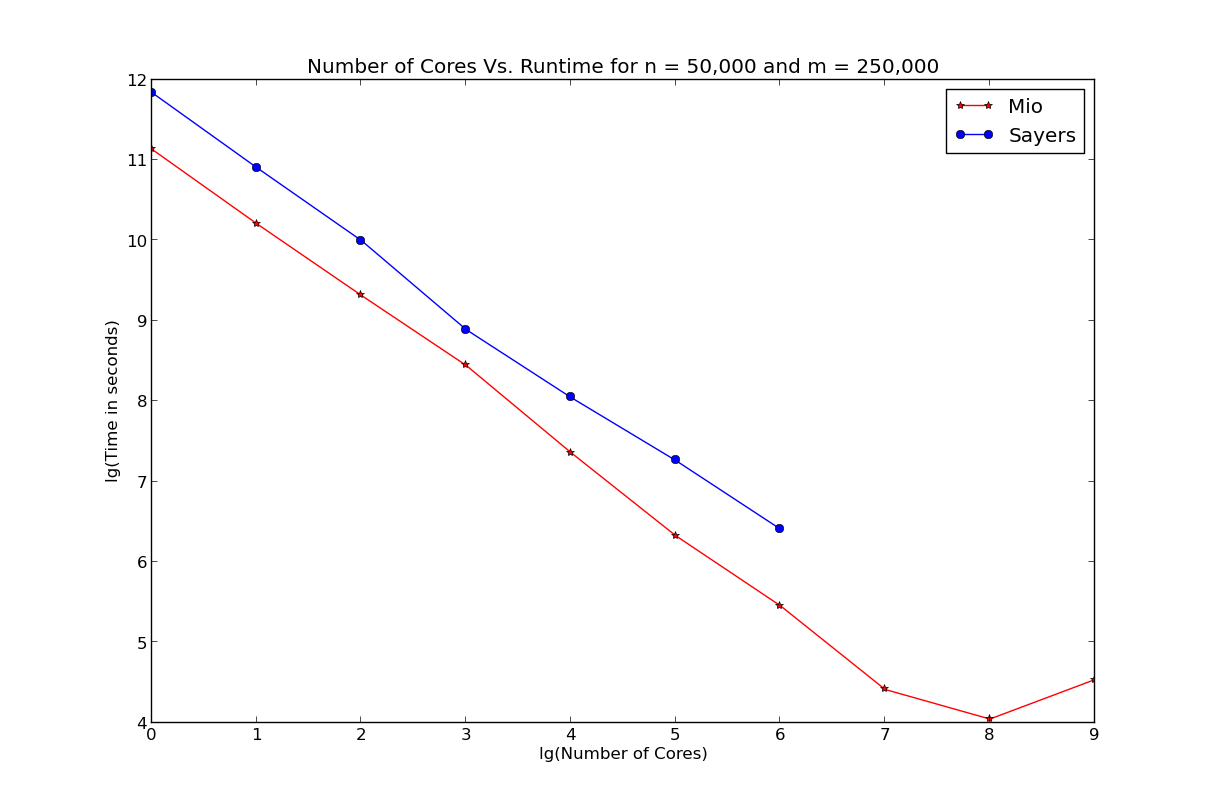
\includegraphics[width=.75\linewidth]{ProjectFiles/results/plots/coresVtime.png}
	
	\subsubsection*{Table 5} \small\textit{Number of cores vs. speedup for $N=50,000$ and $m=250,000$} \\\\
	\normalsize
	\begin{tabular}{r||r|r}
	\hline
  Cores              &Sayers Lab                     &Mio \\ 
	\hline
		  1.0                     &1.0                     &1.0 \\ 
		  2.0      &1.9085366311388137       &1.898990777870678 \\ 
		  4.0      &3.5824280686537624      &3.5265372675142777 \\ 
		  8.0       &7.718560743257858      &6.4486528728878092 \\ 
		 16.0      &13.850570568534692      &13.673355994705298 \\ 
		 32.0      &23.850110244669814      &27.990754393860239 \\ 
		 64.0      &43.125739413179367      &51.233936484810521 \\ 
		128.0                     &N/A      &105.47171583538449 \\ 
		256.0                     &N/A      &136.08431274646915 \\ 
		512.0                     &N/A      &96.940969185966352 \\ 
		\hline
	\end{tabular}
	
	\subsubsection*{Plot 2} \small\textit{Plot of Table $5$ data $(lg(cores)$ vs. $lg(speedup))$} \\
	\normalsize
	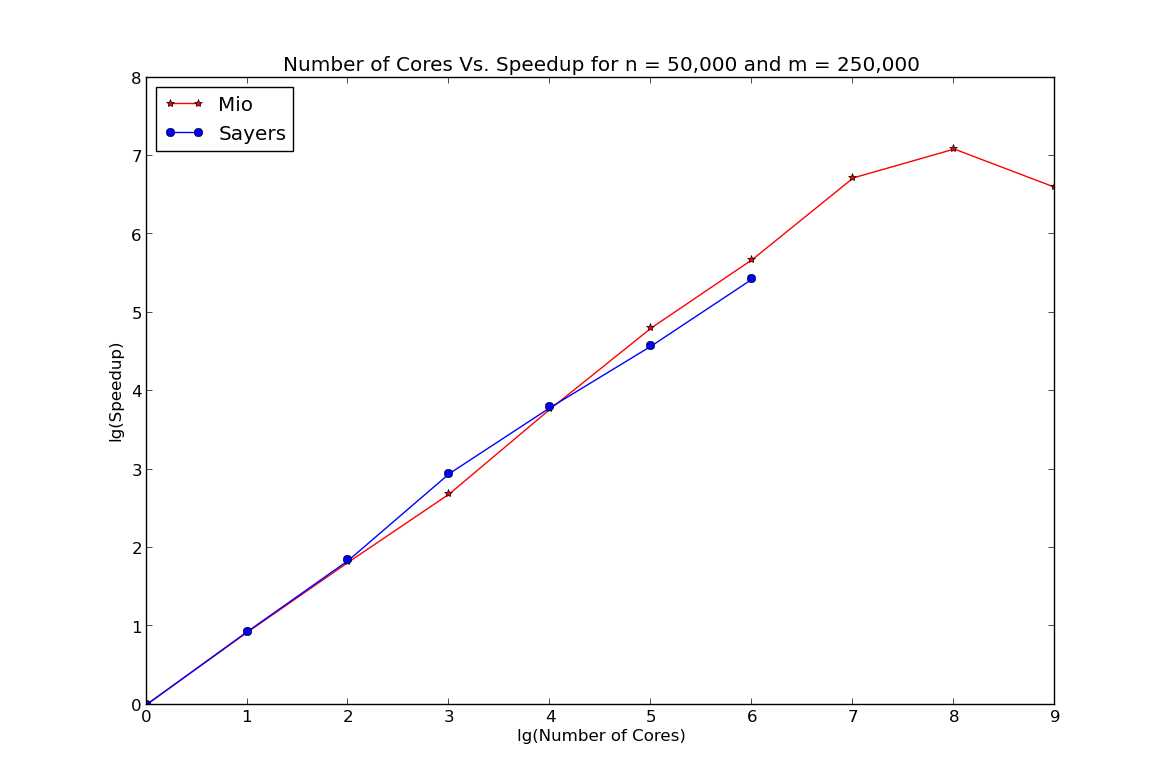
\includegraphics[width=.75\linewidth]{ProjectFiles/results/plots/coresVspeedup.png}
	
	\subsubsection*{Table 6} \small\textit{Number of cores vs. efficiency for $N=50,000$ and $m=250,000$} \\\\
	\normalsize
	\begin{tabular}{r||r|r}
	\hline
		Cores              &Sayers Lab                     &Mio \\ 
	\hline
		  1.0                     &1.0                     &1.0 \\ 
		  2.0     &0.95426831556940683     &0.94949538893533902 \\ 
		  4.0      &0.8956070171634406     &0.88163431687856941 \\ 
		  8.0     &0.96482009290723225     &0.80608160911097615 \\ 
		 16.0     &0.86566066053341828     &0.85458474966908116 \\ 
		 32.0     &0.74531594514593169     &0.87471107480813248 \\ 
		 64.0     &0.67383967833092762     &0.80053025757516438 \\ 
		128.0                     &N/A      &0.8239977799639413 \\ 
		256.0                     &N/A     &0.53157934666589512 \\ 
		512.0                     &N/A     &0.18933783044134053 \\ 
		\hline
	\end{tabular}
	
	\subsubsection*{Plot 3} \small\textit{Plot of Table $6$ data $(lg(cores)$ vs. efficiency$)$} \\
	\normalsize
	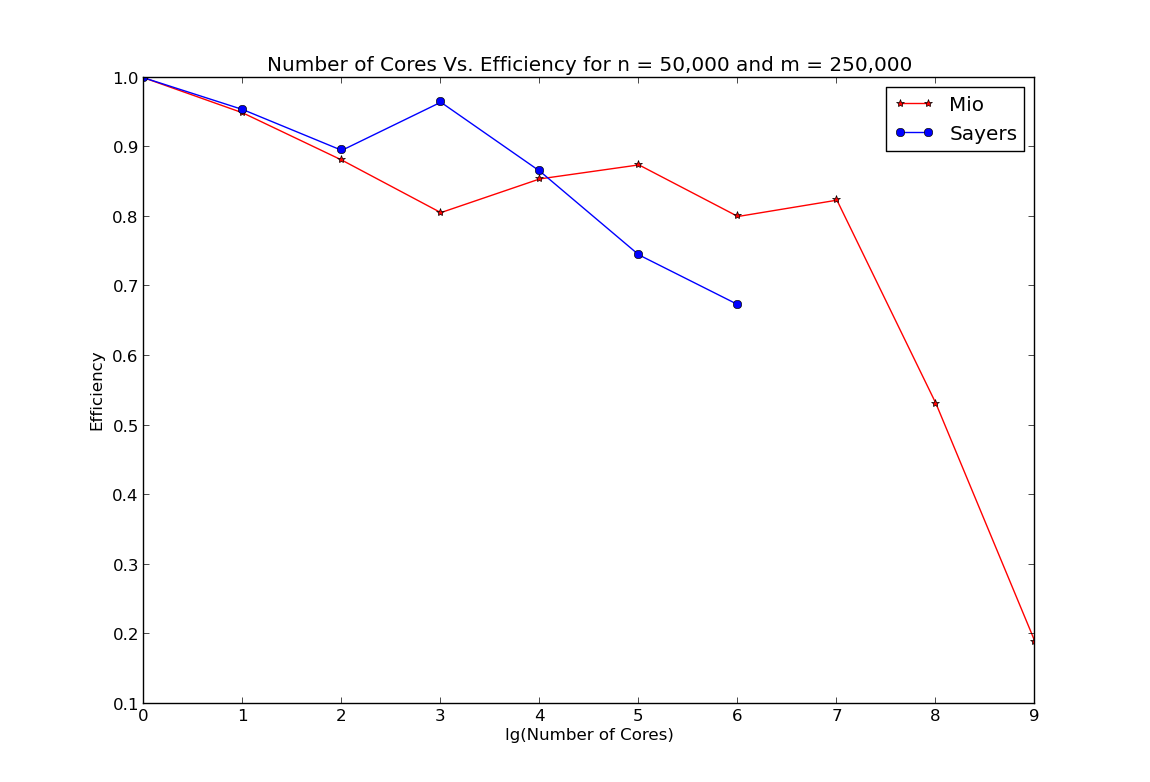
\includegraphics[width=.75\linewidth]{ProjectFiles/results/plots/coresVefficiency.png}
	
	\subsubsection*{Table 7} \small\textit{Number of cores vs. experimental serial fraction of the code for\\ $N=50,000$ and $m=250,000$} \\\\
	\normalsize
	\begin{tabular}{r||r|r}
	\hline
		Cores              &Sayers Lab                     &Mio \\ 
	\hline
		  2.0    &0.047923297551072164    &0.053191001929236759 \\ 
		  4.0     &0.03885371628253953    &0.044752372896321647 \\ 
		  8.0   &0.0052089514409975812    &0.034367025567564609 \\ 
		 16.0    &0.010345804508339492    &0.011343930518085162 \\ 
		 32.0     &0.01102299598743091   &0.0046204722317963586 \\ 
		 64.0   &0.0076830559693734967   &0.0039551114498611187 \\ 
		128.0                     &N/A   &0.0016818543519778373 \\ 
		256.0                     &N/A   &0.0034556341402023306 \\ 
		512.0                     &N/A   &0.0083787958735268026 \\ 
		\hline
	\end{tabular}
	
	\subsubsection*{Plot 4} \small\textit{Plot of Table $7$ data $(lg(cores)$ vs. experimental serial fraction of the code$)$} \\
	\normalsize
	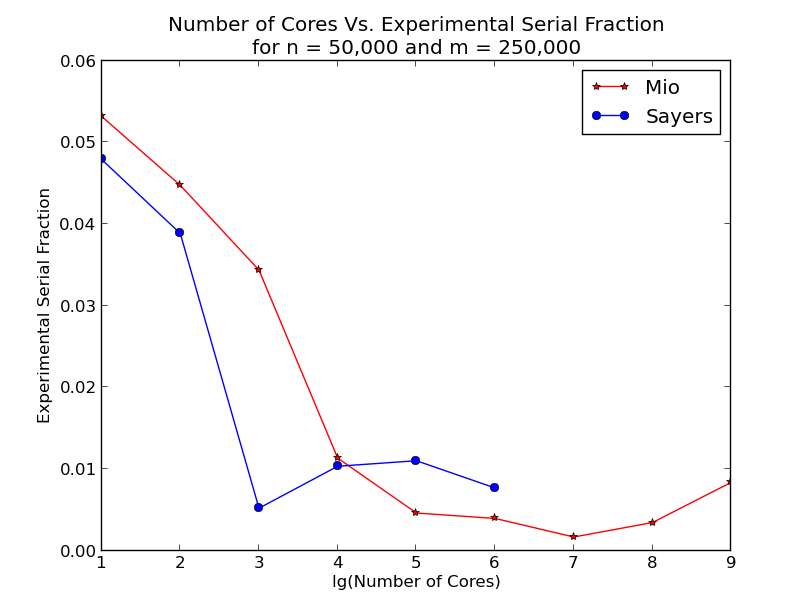
\includegraphics[width=.75\linewidth]{ProjectFiles/results/plots/coresVexpserialfrac.png}
	
	\begin{thebibliography}{1}
		\bibitem{sheen03}
			Dongwoo Sheen, Ian H. Sloan, and Vidar Thom\'{e}e,
			\emph{A parallel method for time discretization of parabolic equations based on Laplace transformation and quadrature}.
			IMA Journal of Numerical Analysis (2003) 23,
			269-299
			
	\end{thebibliography}
	
	 % nice mathy stuff for our presentation
 
 $$U_{N,\tau}(t)=2\text{Re}\left(\frac{1}{N\tau}\sum_{j=0}^{N-1}{}^\prime \tilde{\mu_j}\e^{z_jt}w(z_j)\right)$$
 $$(zI+A)w(z)=u_0+\hat{f}(z)$$
 $$u_t+Au=f(t),\hspace{4mm}\text{for }t>0,\hspace{4mm}\text{with }u(0)=u_0$$
 $$u_t-u_{xx}=f(x,t),\hspace{4mm}\text{for }0<x<\pi,\;t>0,$$
 $$u(x,t)=0\hspace{4mm}\text{for }x=0\text{ and }\pi,\;t>0,\hspace{4mm}\text{with }u(x,0)=u_0(x),\hspace{4mm}\text{for }0<x<\pi$$
 $$u(x,t)=(1+t)\e^{-t}\sin(x)+\cos(t)\e^{-2t}\sin(2x)$$
 $$u_0(x)=\sin(x)+\sin(2x)$$
 $$\hat{f}(x,z)=\frac{1}{1+z}\sin(x)+\frac{2z+3}{(z+2)^2+1}\sin(2x)$$
 
 % end nice mathy stuff

\end{document}
